\documentclass{deliverablereport}

\deliverable{UI}{jupyter-live-collab}
\deliverydate{31/08/2018}
\duedate{31/08/2018 (M36)}
\author{Benjamin Ragan-Kelley, Vidar Tonaas Fauske}

\begin{document}
\maketitle
\tableofcontents

%%%%%%%%%%%%%%%%%%%%%%%%%%%%%%%%%%%%%%%%%%%%%%%%%%%%%%%%%%%%%%%%%%%%%%%%

\section{Introduction}

The \href{https://jupyter.org}{Jupyter Notebook} is a web application
that enables the creation and sharing of executable documents
containing live code, equations, visualizations and explanatory text.
One of the main uses of Jupyter is as an interactive computing environment,
building interactive notebook documents.
\taskref{UI}{notebook-collab} is focused on improving the process of collaborating
on Jupyter notebooks in the various ways researchers and educators use them.
\delivref{UI}{jupyter-collab} improved collaborating on notebooks via traditional version-control systems.

This deliverable aims to improve the process of ``live collaboration'' on notebook documents,
where two authors on different computers are editing the same document at the same time,
and they are kept in sync over the internet.

There have been prior efforts to enable live collaboration on notebooks,
notably \href{https://colaboratory.google.com}{Google Colaboratory}
and \href{https://cocalc.com}{CoCalc} (formerly SageMathCloud).
These efforts added live collaboration on notebooks to an existing,
fully hosted cloud service.
CoCalc can be downloaded and run as free, open source software,
but not integrated into existing deployments of notebooks.
Our goal is to learn from these examples and build an official live collaboration implementation into the JupyterLab notebook application,
so that it can be available to all Jupyter users,
developed in collaboration with the Jupyter community.


The target usage scenario for this effort is two users having access to the same hosted notebook server, e.g. hosted with JupyterHub,
being able to view and edit the document at the same time.
Example applications include researchers co-authoring an analysis
or an instructor helping a student through examples.
This should require no additional infrastructure,
and not rely on any commercial hosted service.
In particular, it should be able to be used anywhere that Jupyter is already used,
without opting into other systems.
This last point will be the primary differentiator for the official Jupyter implemntation,
as opposed to those currently existing in hosted services.

%%%%%%%%%%%%%%%%%%%%%%%%%%%%%%%%%%%%%%%%%%%%%%%%%%%%%%%%%%%%%%%%%%%%%%%%

\section{Prototyping}

The Jupyter Community has developed a first prototype of live collaboration in JupyterLab,
prior to \ODK involvement.
This implementation relied on the Google real-time documents API and storing notebook documents in Google Drive.
By relying on an existing implementation of a real-time server and storage,
development could focus on making JupyterLab's
internal models and APIs suitable for real-time collaboration.
In 2017, Google deprecated this API and it can no longer be used,
but the lessons learned from this prototype have been useful in guiding JupyterLab design to best fit a real-time collaboration model.

\ODK participation began with the next stage, designing a full real-time collaboration prototype
that does not rely on any external hosting provider,
such as Google.
This work was carried out in close collaboration with the Jupyter developer community.
There are many participants in this effort, and \ODK has contributed approximately
three person-months to the design and implementation of real-time collaboration in JupyterLab.

\TODO{Ensure reasonable scale of PDF fig, maybe adjust font size?}

\begin{figure}[h]
  \centering
  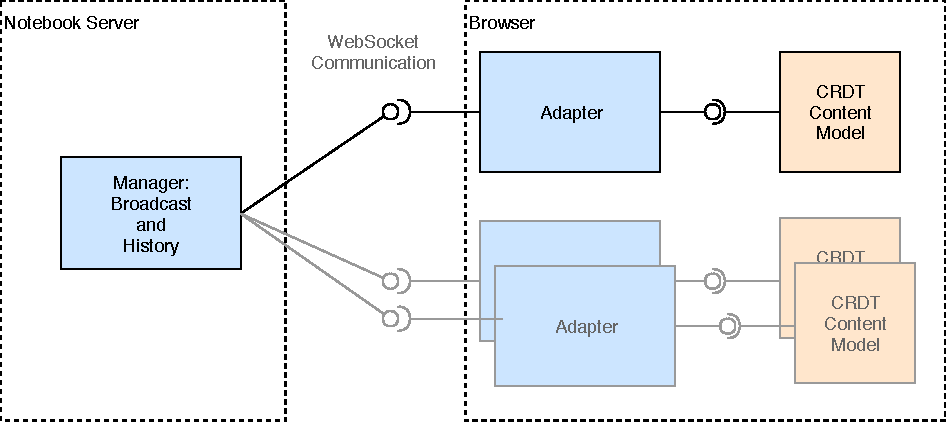
\includegraphics[scale=0.6]{lab-RTC.pdf}
  \caption{A schematic overview of the currently planned real time collaboration components.
    Light blue components should be implemented in JupyterLab, while the beige
    components (CRDT models) should be implemented in PhosphorJS.}
  \label{fig:rtc-components}
\end{figure}

The current road map specifies an implementation build on top of
\emph{conflict-free replicated data types} (CRDTs). The implementation outlines the
following components: a client side implementation of the CRDTs; a client side interface
for broadcasting these changes to other consumers; a wire protocol for broadcasting
changes and requesting history over the network; and a notebook server extension for broadcasting changes. See Figure~\ref{fig:rtc-components} for a schematic overview.

So far, the wire format for communicating and requesting changes and history has been
agreed, and proof of concept implementations for the transmission and receipt of the
wire format have been completed. Work is ongoing in the PhosphorJS project to implement
efficient client side CRDTs.


\section{Challenges and status}

The biggest challenge for \ODK participation in JupyterLab is that it is a large collaboration, driven by many interests,
often where one task must wait for another to be completed.
Real-time collaboration is of interest to many involved,
but relies on significant changes of underlying datastructures in JupyterLab before implementation can proceed.

While we have not yet delivered a fully working production implementation of real-time collaboration,
we have laid the groundwork and assembled prototypes and an implementation plan
in collaboration with the JupyterLab team,
and we are optimistic that our remaining resources will enable us to help deliver a working implementation integrated into JupyterLab by the completion of \taskref{UI}{notebook-collab}.

\end{document}
